\documentclass[11pt,a4paper]{article}
\usepackage{freshaudit}
\usepackage{pdfpages}
\usepackage{bookmark}

\title{Glimm--Jaffe Parts I and II\\[4pt]
\large Complete Lamport-notation reconstruction of the current proof chain}
\author{Fresh independent reconstruction and adversarial audit}
\date{16 August 2026}

\begin{document}
\maketitle

\begin{resultbox}
This volume expands the canonical Part I manuscript and the current Part II proof
chain into numbered Lamport-style steps.  It incorporates the explicit repairs
identified by the accompanying critical audit; it is therefore both a reconstruction
and a precise statement of what would have to replace the defective passages in the
source files.
\end{resultbox}

\section*{How to read this volume}

The reconstruction is modular because the underlying Part II argument is modular.
Every module is a separately compilable document with its own definitions and
dependency interface; the remainder of this volume binds the resulting PDFs without
altering their page images.  The source manuscripts themselves were not silently
rewritten.

The verdicts are deliberately asymmetric:

\begin{itemize}
\item Part I is \Conditional.  Its internal chain is valid after localizing the CE2
application cell by cell, but the claimed cutoff-uniform GJS scope remains an explicit
external import rather than a reproduced cluster expansion.
\item Part II is \Fail{} as written in the original V2 file: the assertion excluding
four edge modes is false, and the shifted comparison drops an undefined remainder.
The V2 module in this volume supplies the exact four-edge contribution and a complete
fundamental-band/alias repair.  With those replacements, V3--V4 close at the claimed
rates.
\end{itemize}

The separate \emph{Critical audit of Parts I and II} gives the finding-by-finding
verdict, while the separate \emph{Citation evidence dossier} reproduces every
source page used to assess an imported statement.  These three documents should be
read together.

\section*{Module order and coverage}

\begin{longtable}{P{1.0cm}P{5.1cm}P{7.6cm}}
\toprule
Part & Module & Coverage \\
\midrule
\endhead
I & Euclidean input to the Hamiltonian gap & Slab FKN representation, GJS clustering
inputs, localized CE2 repair, dense polynomial vectors, and the gap inequality. \\
I & Gap to the main theorem & Path differentiability, inverse-energy filter,
separation and clustering, one-path LPPL, full local norm convergence, local
normality, spectral passage, invariances, and the conditional phase conclusion. \\
II & Model sheet & Lattices, Weyl embeddings, Hamiltonians, closed coercive forms,
compactness, ground-state simplicity, and Wick constants. \\
II & Quadratic obstruction & Exact finest-scale covariance obstruction and its
consequences for naive continuum comparison. \\
II & Projective compactness & Cofinal compactness, consistency, and the distinction
between subsequential and identified full-sequence limits. \\
II & Free fixed-coarse rate & D4 filter envelope/telescope, dispersion estimates,
low/high-frequency split, and quantitative free convergence. \\
II & Weyl reduction & Pointwise Weyl criterion, extension to the coarse algebras,
inductive-limit identification, and symmetry. \\
II & Gate scoping & Minimal gate logic, the sharp-time momentum-source no-go theorem,
the mean-shift amendment, A1--A8 dependency map, and rejection of the slab fallback as
load bearing. \\
II & V1 & Weyl action, trace kernel, oscillator trace, Mehler bridge, exact jump
shift, interacting marked-slice formula, continuum free formula, and thermal free
rate. \\
II & V2 & Same-noise coupling, edge covariance, Wick/convolution estimates,
unshifted comparison with the four-edge correction, Wick dictionary, exact shifted
fundamental-band/alias comparison, and Nelson bounds. \\
II & V3 & Continuum interaction, uniform exponential bounds, finite-mode FKN,
strong semigroup construction, generator/form identification, trace class and
trace-norm approximation, periodic insertions, positivity improvement, and the gap. \\
II & V4 & Coupled thermal comparison, normal-ordered partition convergence, full
Laplace spectral transfer, derived lattice gap, thermal-to-ground interchange, gate,
inductive-limit identification, and $\mathbb Z_2$ symmetry. \\
\bottomrule
\end{longtable}

\clearpage
\tableofcontents
\clearpage

\part*{Part I}
\addcontentsline{toc}{part}{Part I}

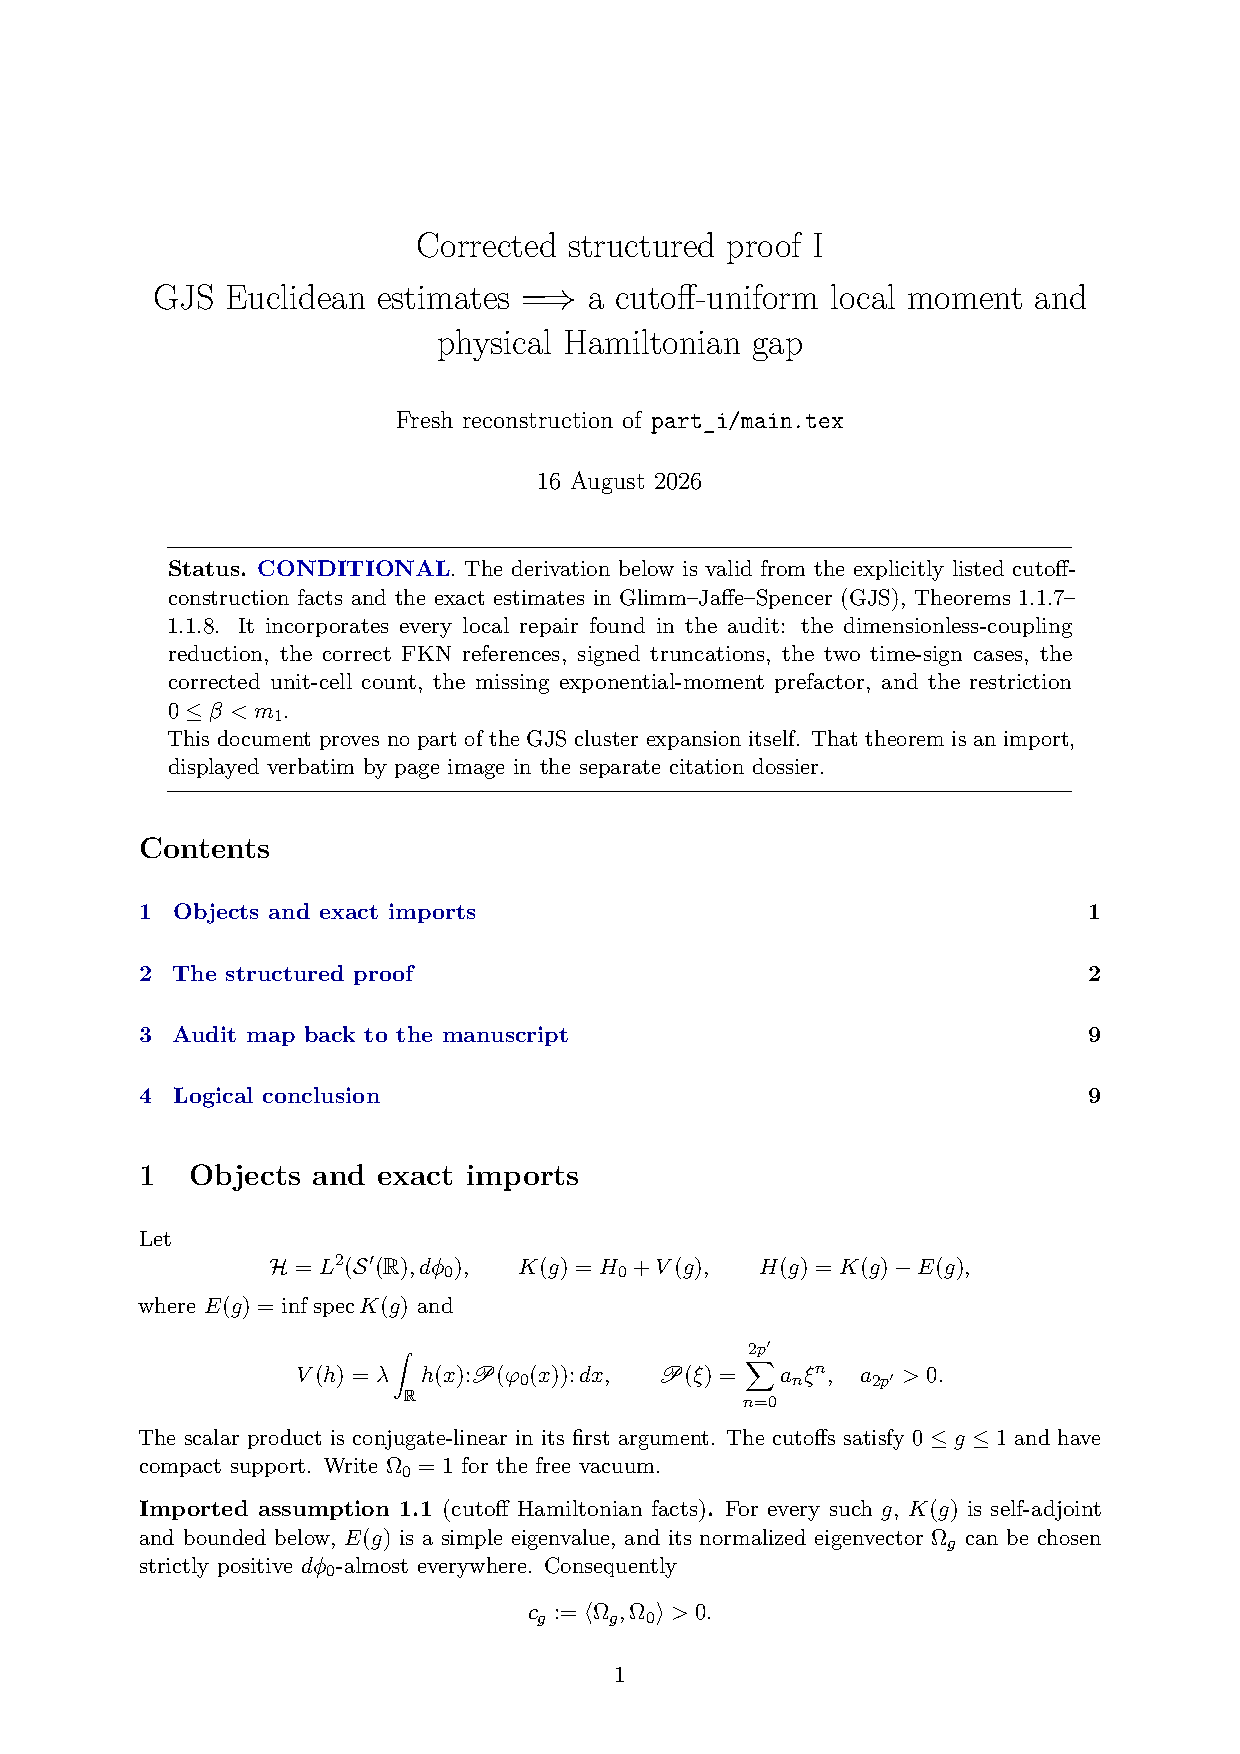
\includepdf[pages=-,pagecommand={\thispagestyle{empty}},addtotoc={1,section,1,
{Part I: Euclidean input to the Hamiltonian gap},mod:i-euclidean-gap}]
{lamport/part_i_euclidean_to_gap.pdf}

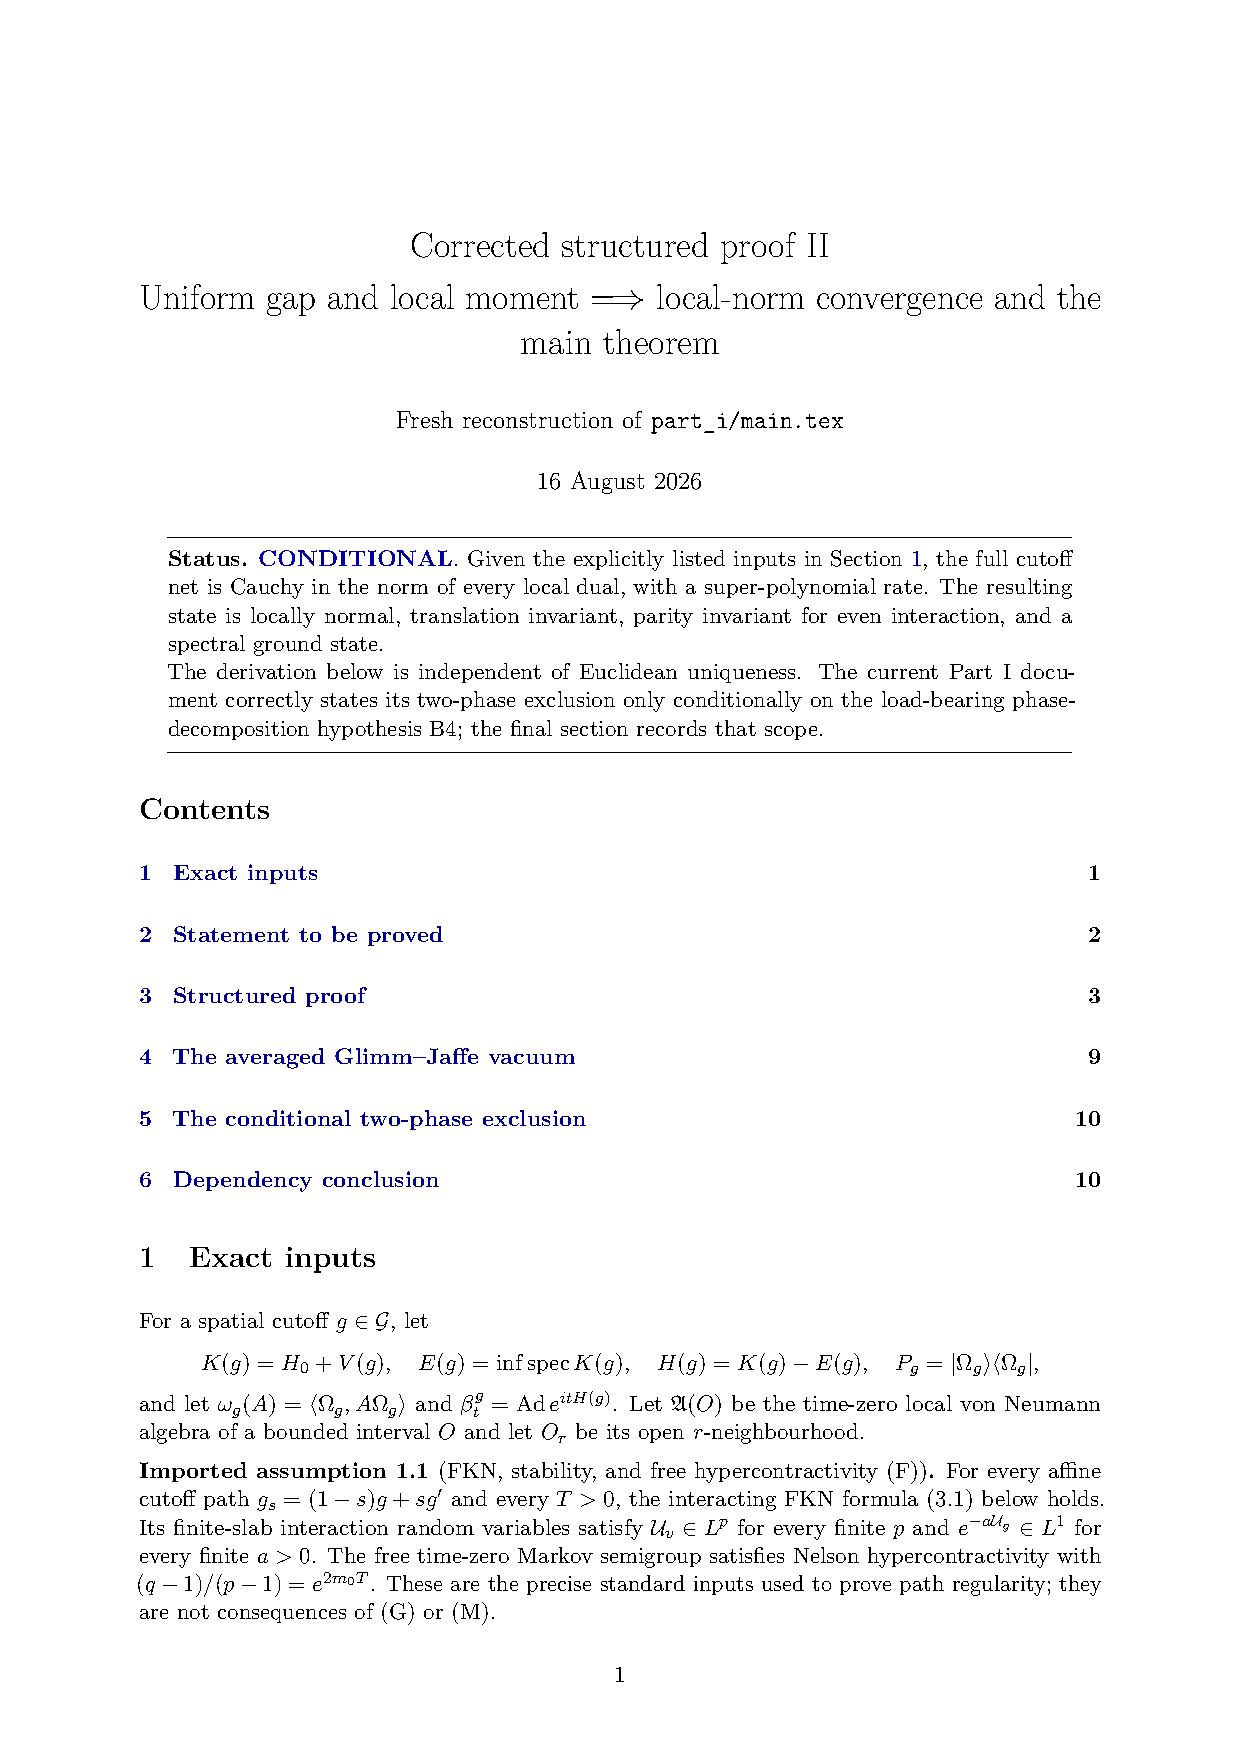
\includepdf[pages=-,pagecommand={\thispagestyle{empty}},addtotoc={1,section,1,
{Part I: From the gap to the main theorem},mod:i-gap-main}]
{lamport/part_i_gap_to_main.pdf}

\part*{Part II}
\addcontentsline{toc}{part}{Part II}

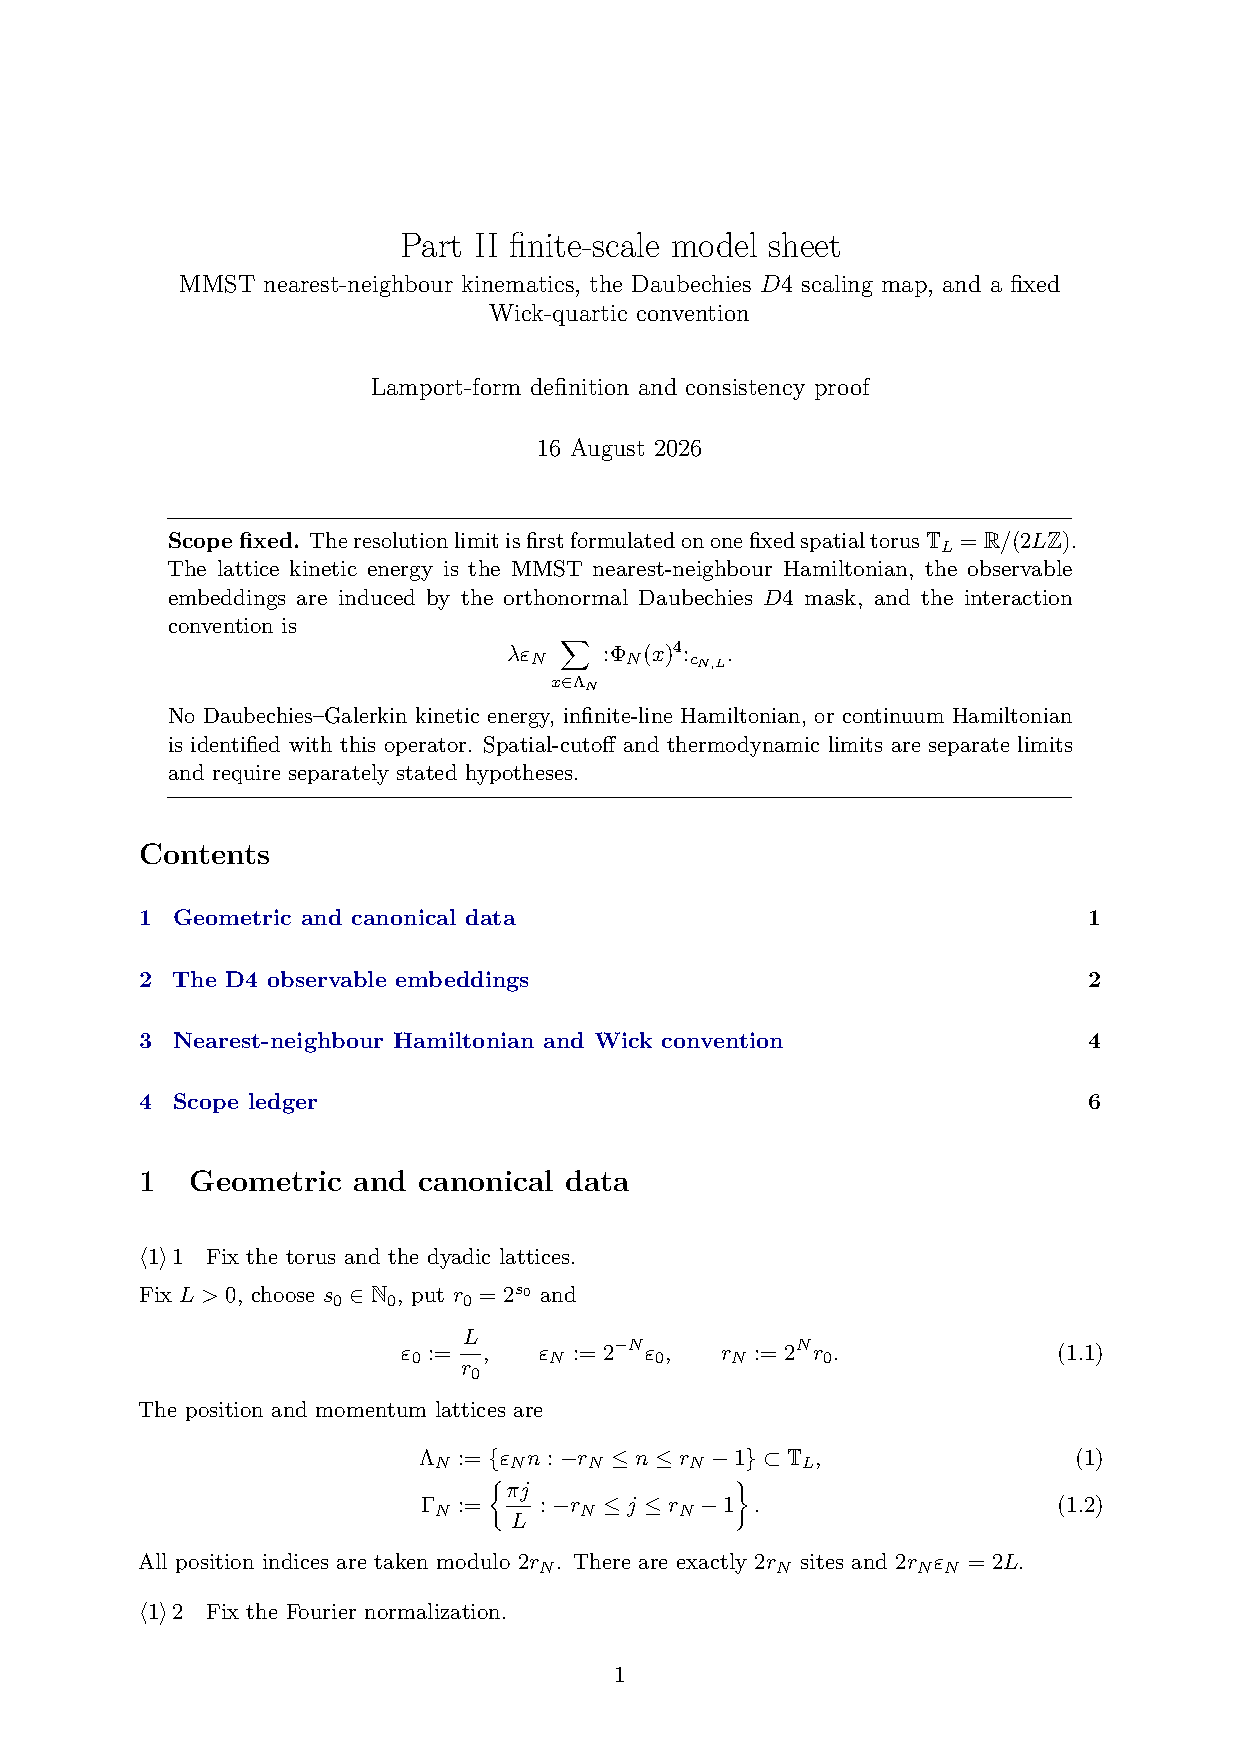
\includepdf[pages=-,pagecommand={\thispagestyle{empty}},addtotoc={1,section,1,
{Part II: Model sheet},mod:ii-model}]
{lamport/part_ii_model_sheet.pdf}

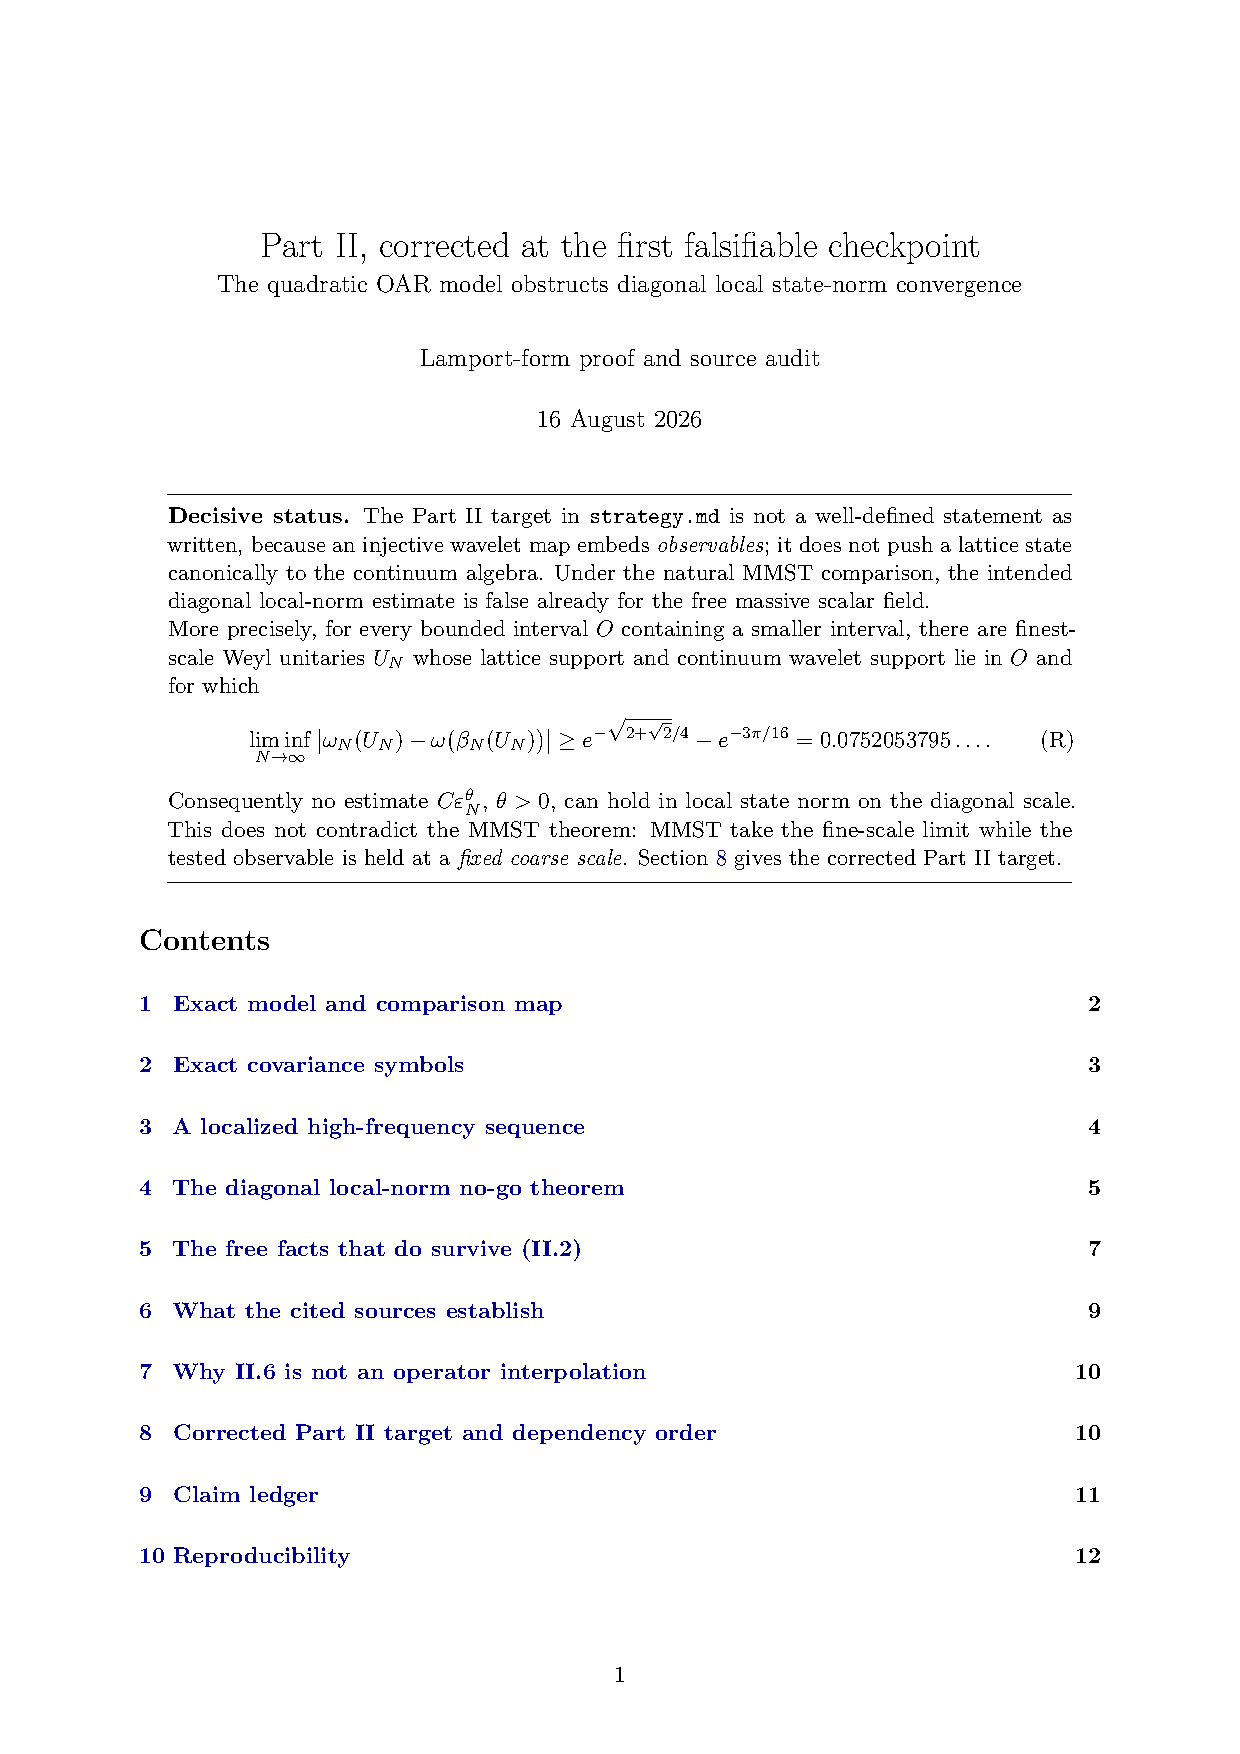
\includepdf[pages=-,pagecommand={\thispagestyle{empty}},addtotoc={1,section,1,
{Part II: Quadratic obstruction},mod:ii-obstruction}]
{lamport/part_ii_quadratic_obstruction.pdf}

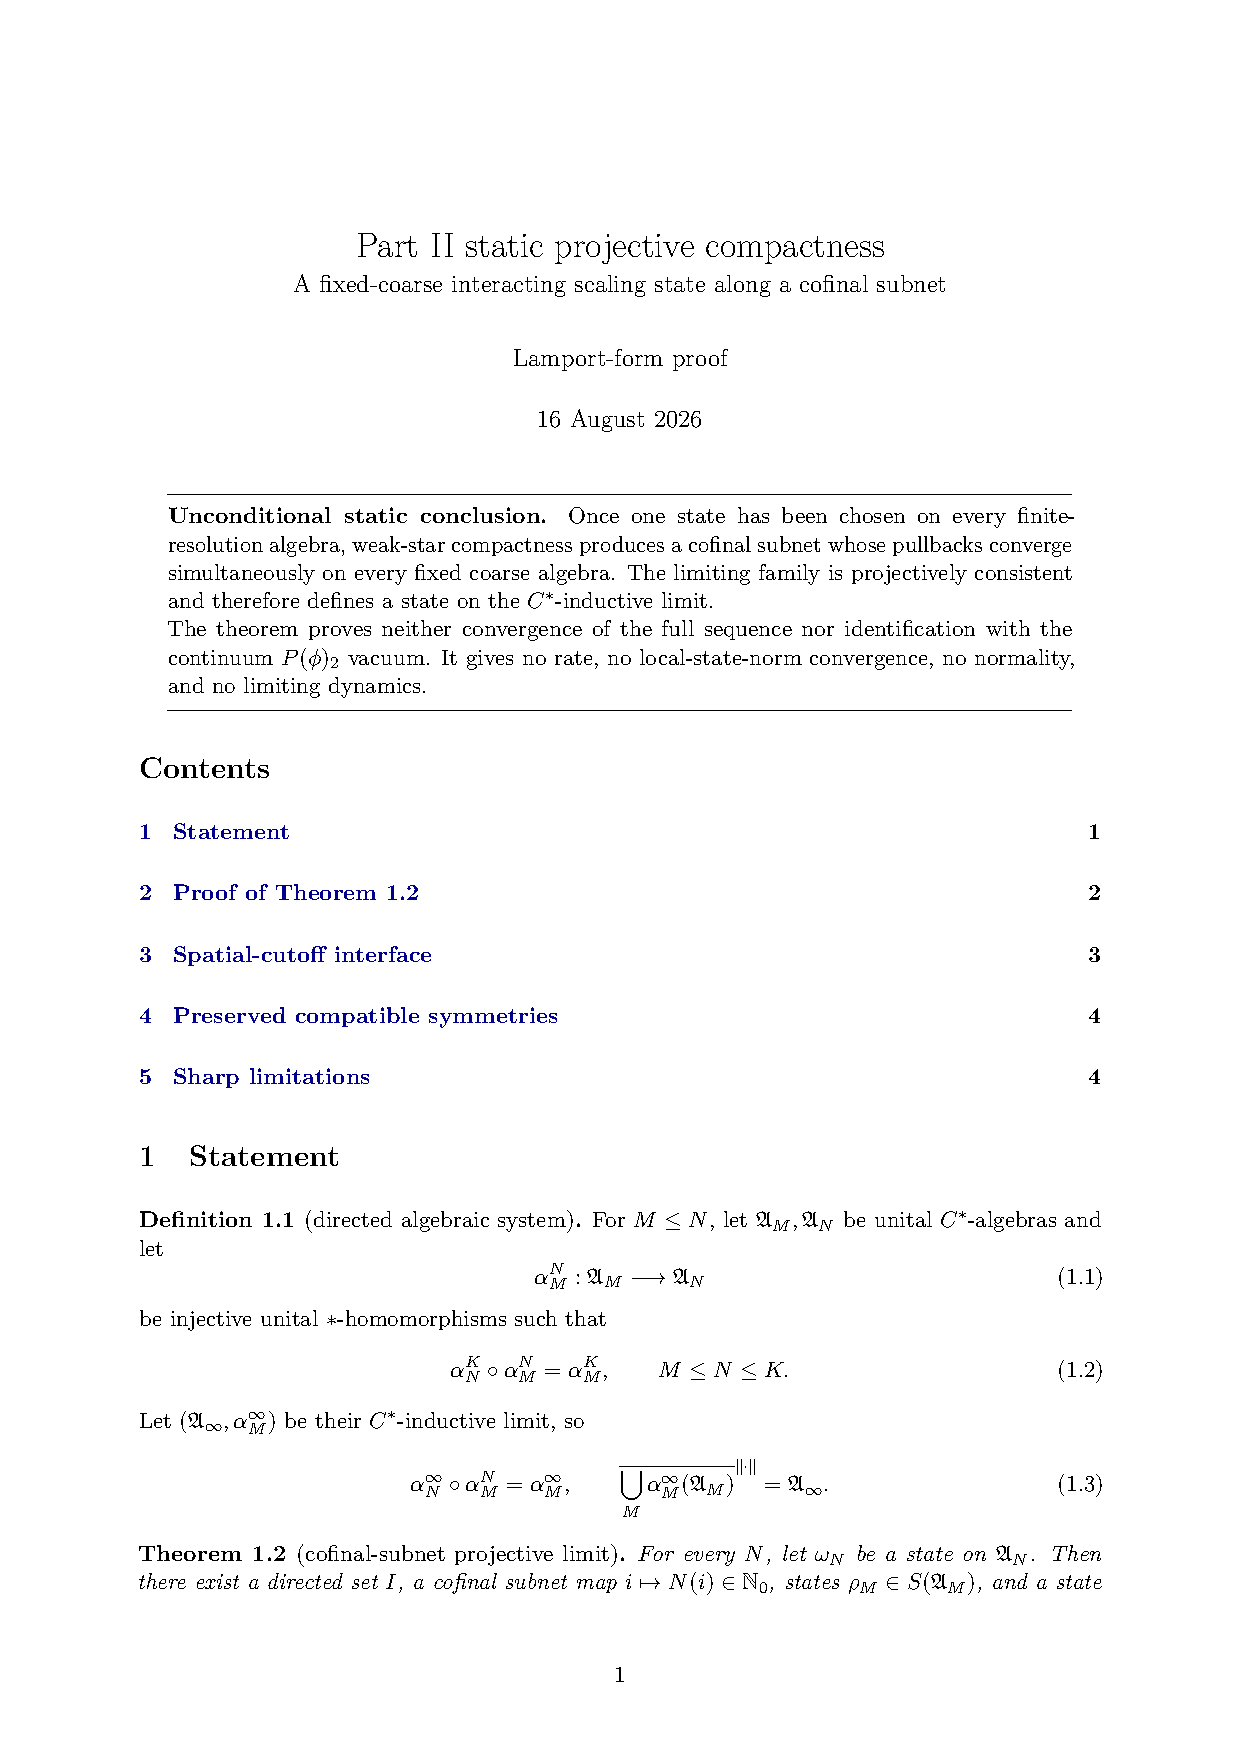
\includepdf[pages=-,pagecommand={\thispagestyle{empty}},addtotoc={1,section,1,
{Part II: Projective compactness},mod:ii-projective}]
{lamport/part_ii_projective_compactness.pdf}

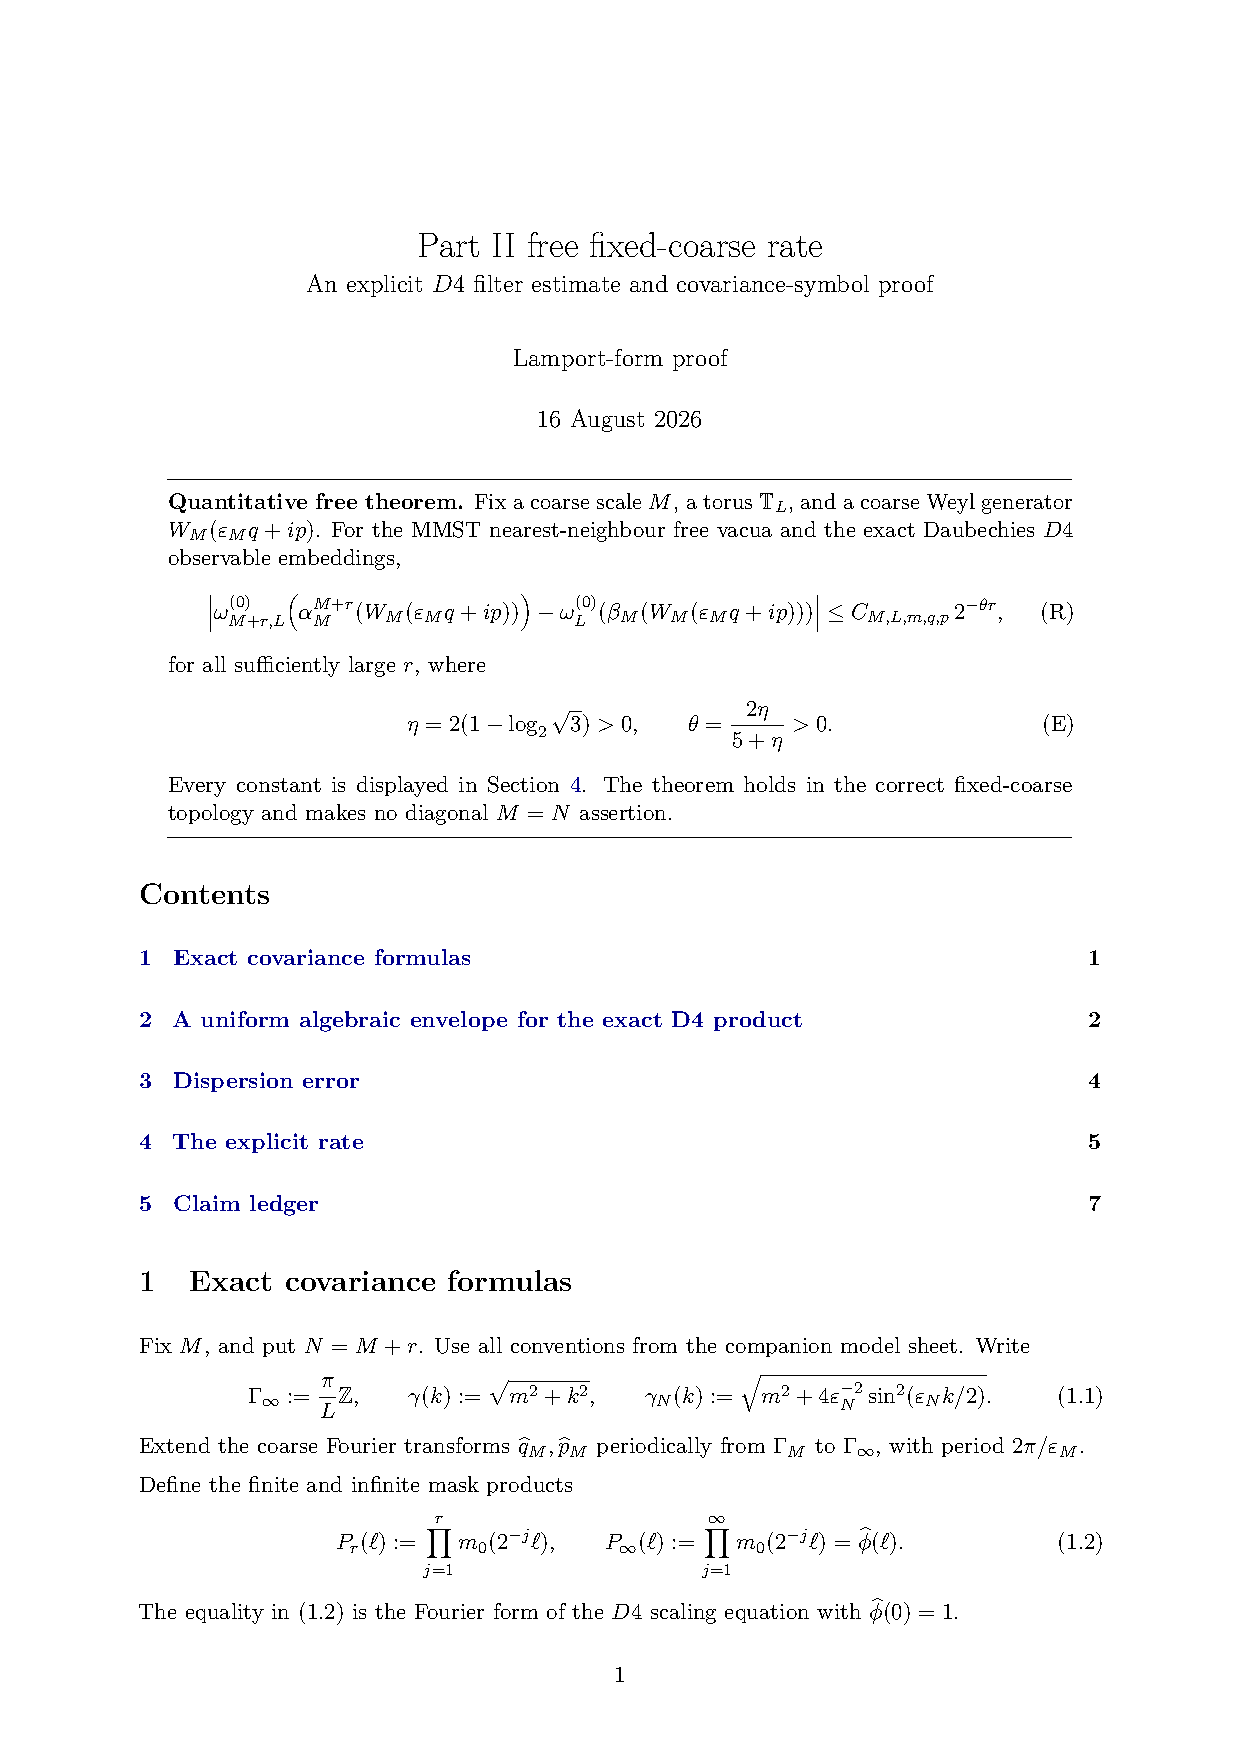
\includepdf[pages=-,pagecommand={\thispagestyle{empty}},addtotoc={1,section,1,
{Part II: Free fixed-coarse rate},mod:ii-free-rate}]
{lamport/part_ii_free_fixed_coarse_rate.pdf}

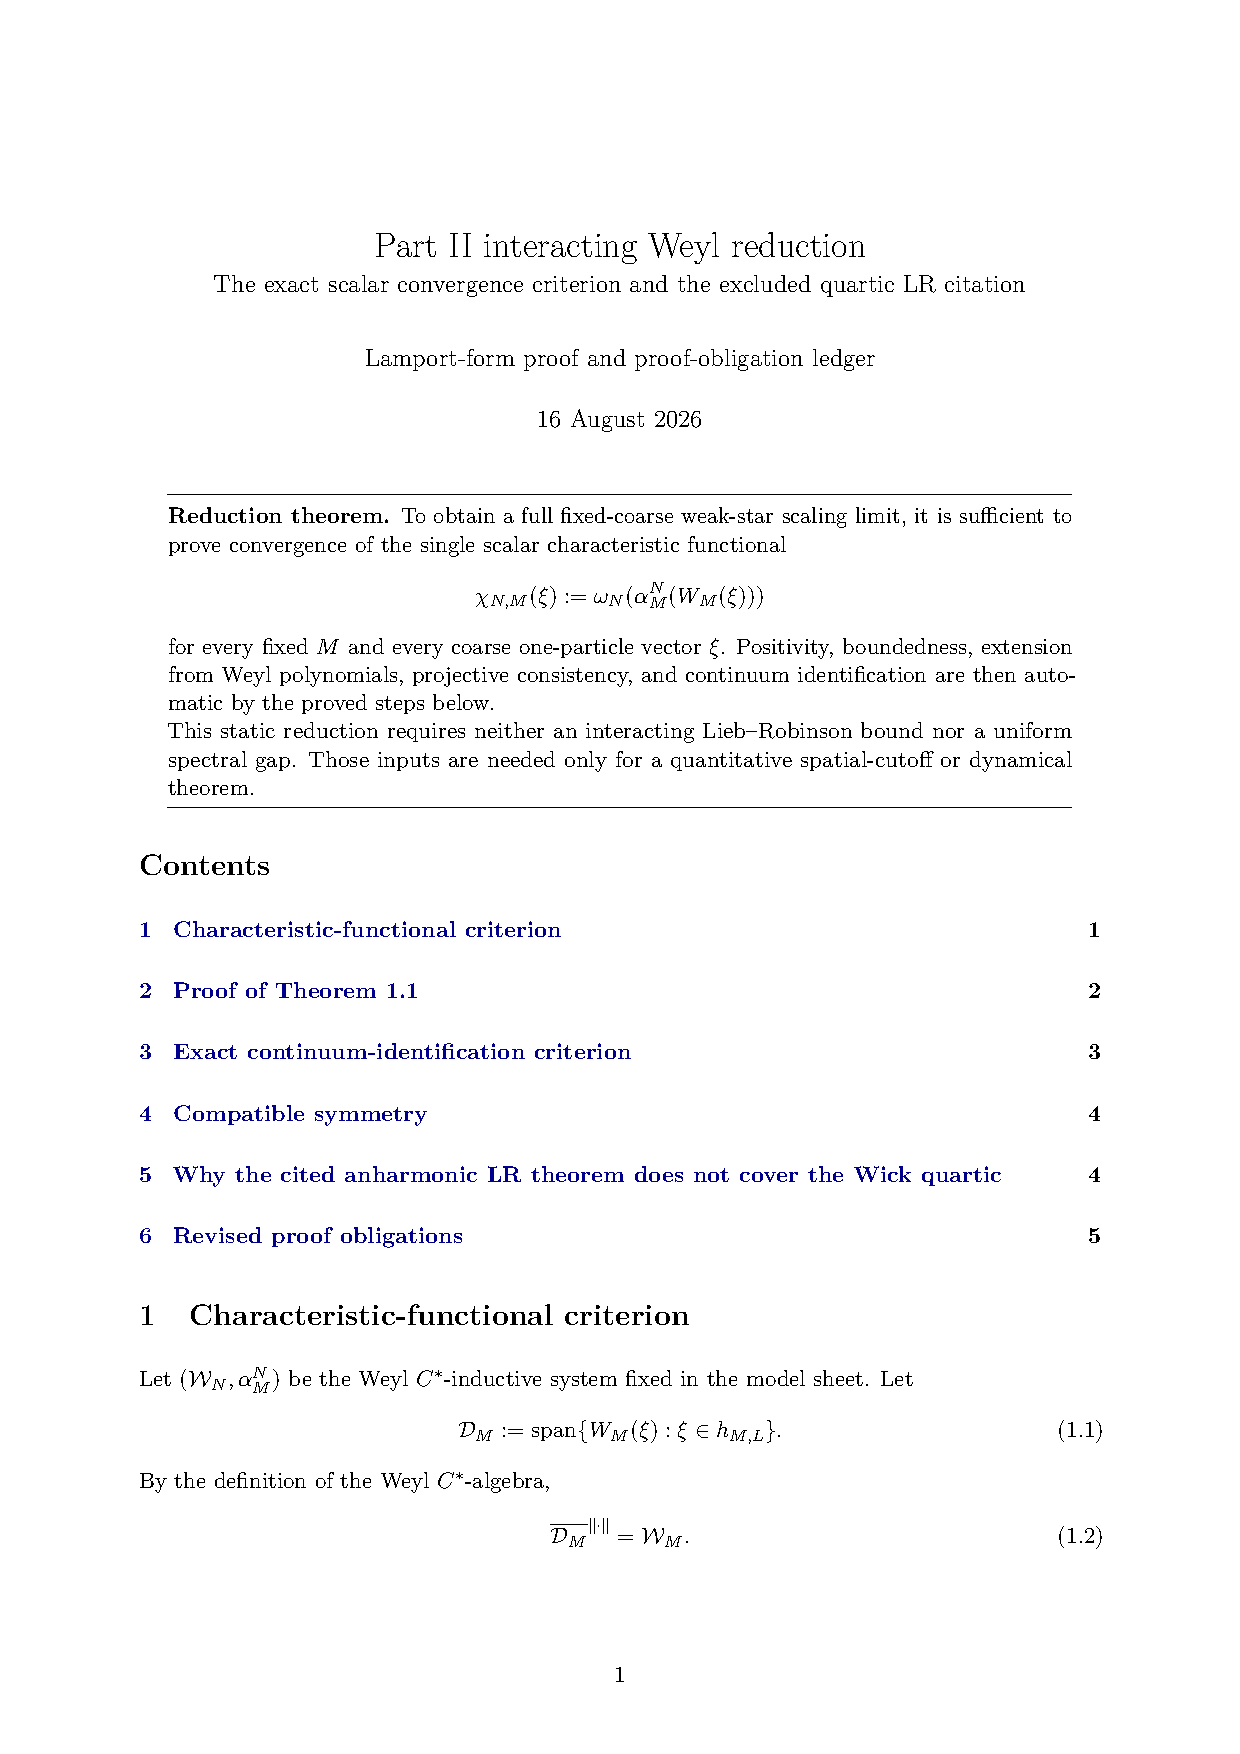
\includepdf[pages=-,pagecommand={\thispagestyle{empty}},addtotoc={1,section,1,
{Part II: Weyl reduction},mod:ii-weyl}]
{lamport/part_ii_weyl_reduction.pdf}

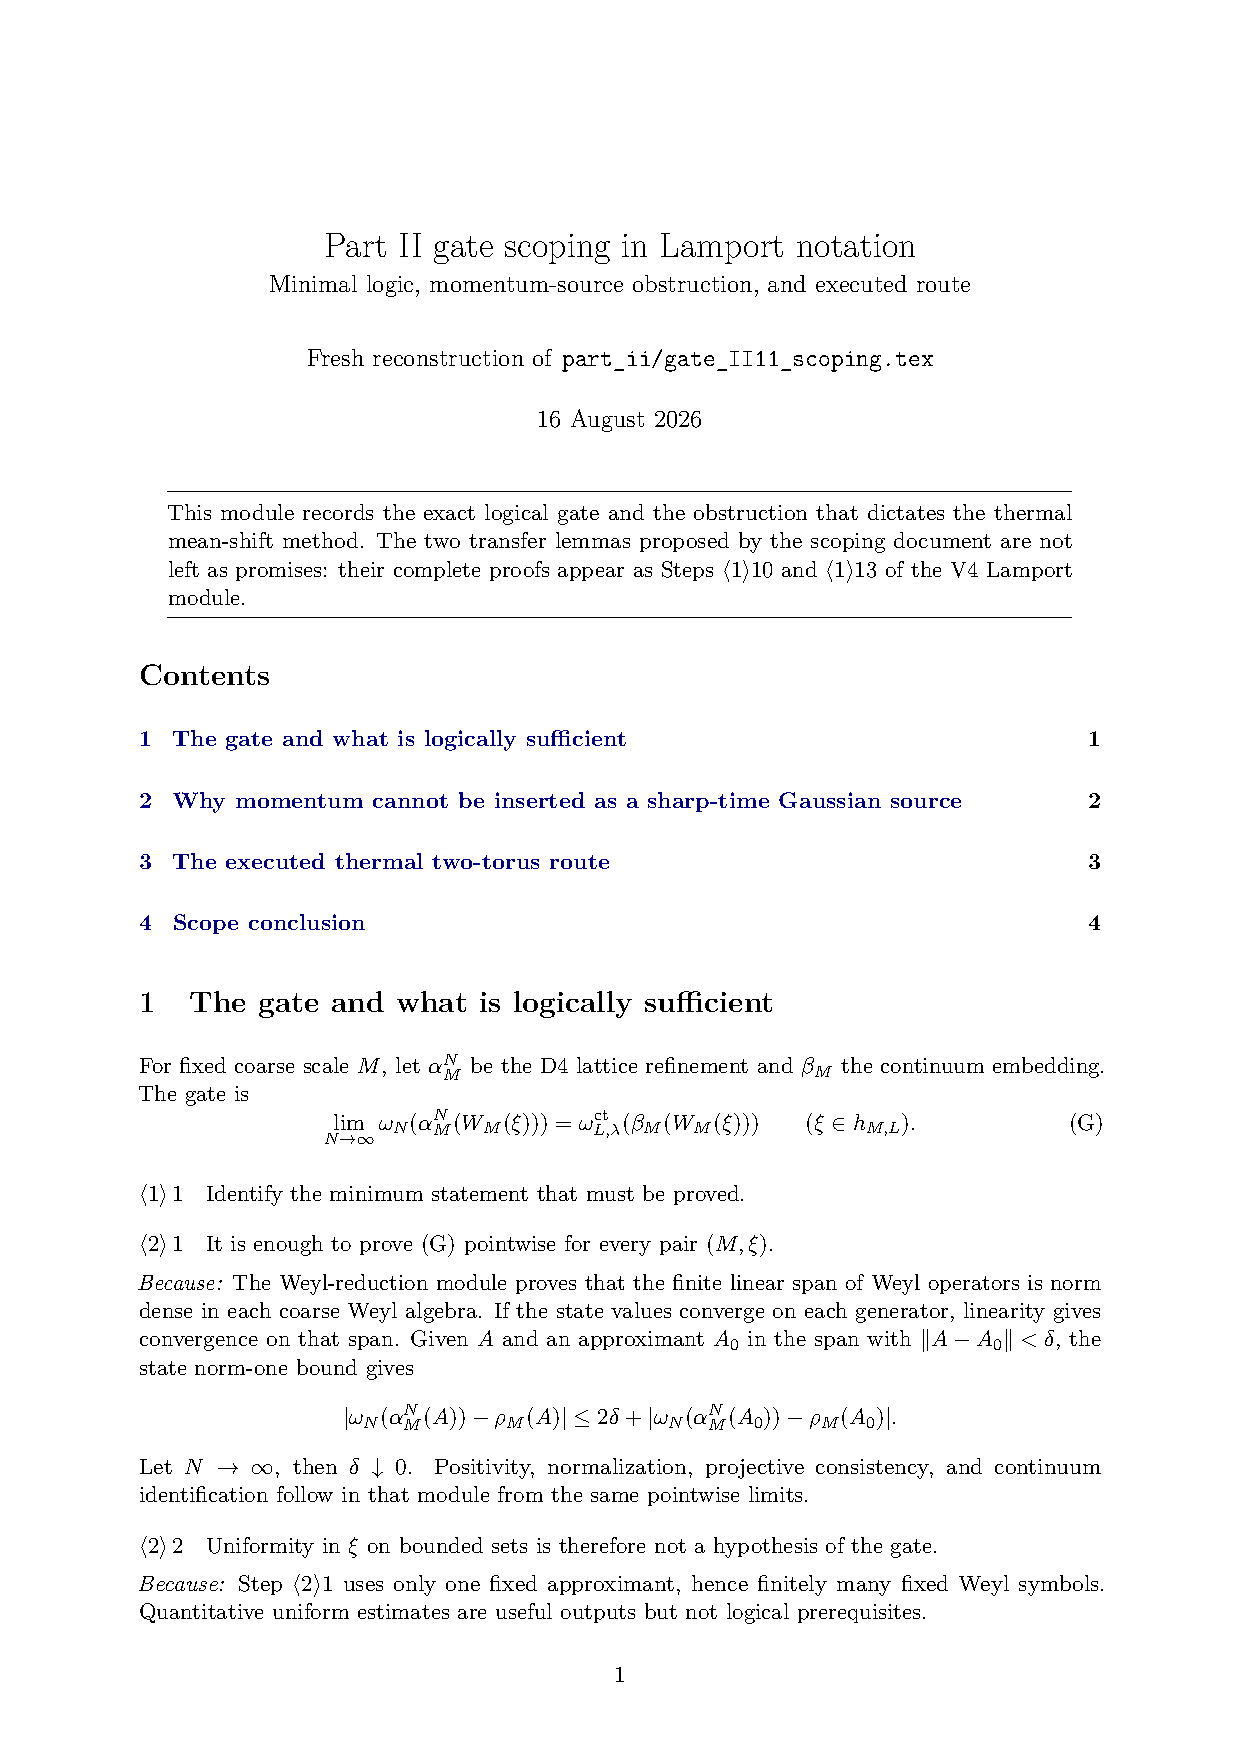
\includepdf[pages=-,pagecommand={\thispagestyle{empty}},addtotoc={1,section,1,
{Part II: Gate scoping and momentum-source obstruction},mod:ii-scope}]
{lamport/part_ii_gate_scoping.pdf}

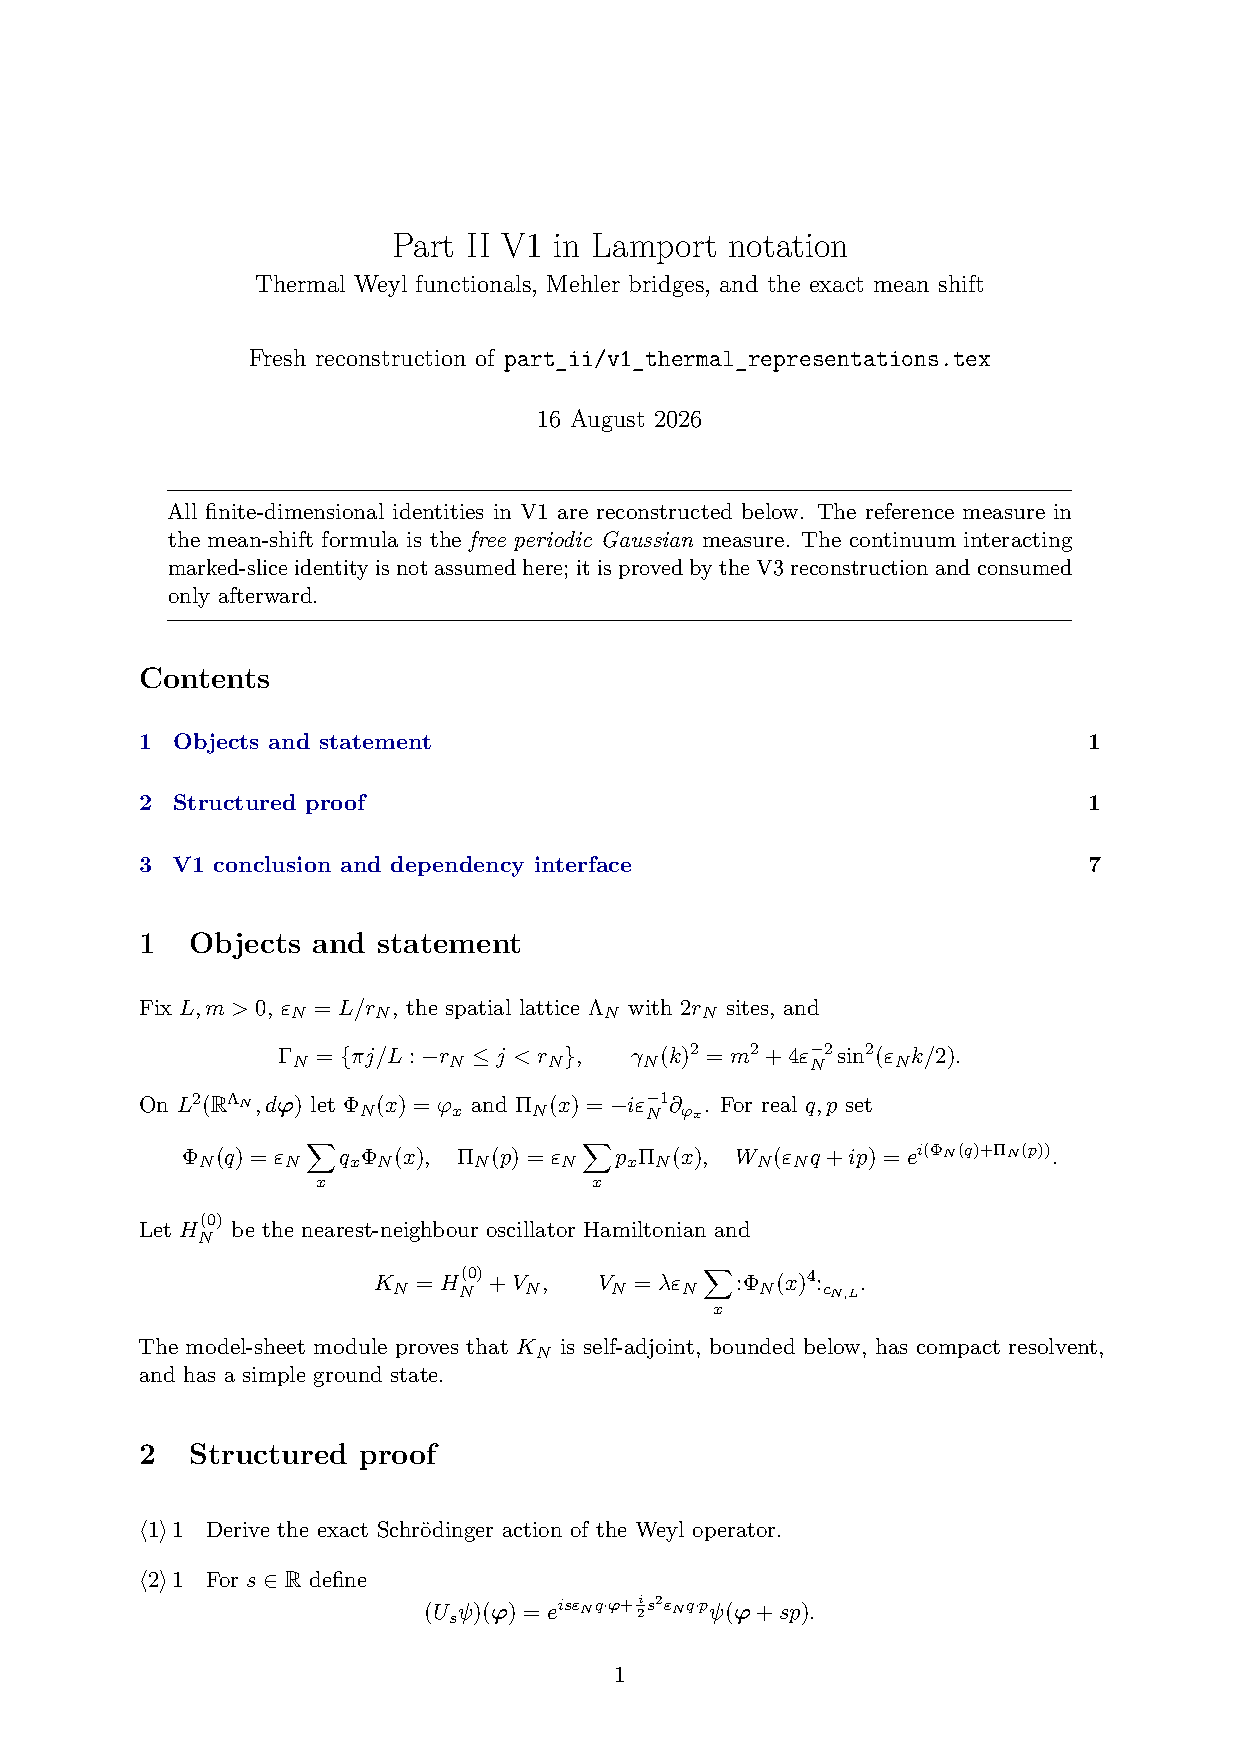
\includepdf[pages=-,pagecommand={\thispagestyle{empty}},addtotoc={1,section,1,
{Part II V1: Thermal representations},mod:ii-v1}]
{lamport/part_ii_v1_thermal.pdf}

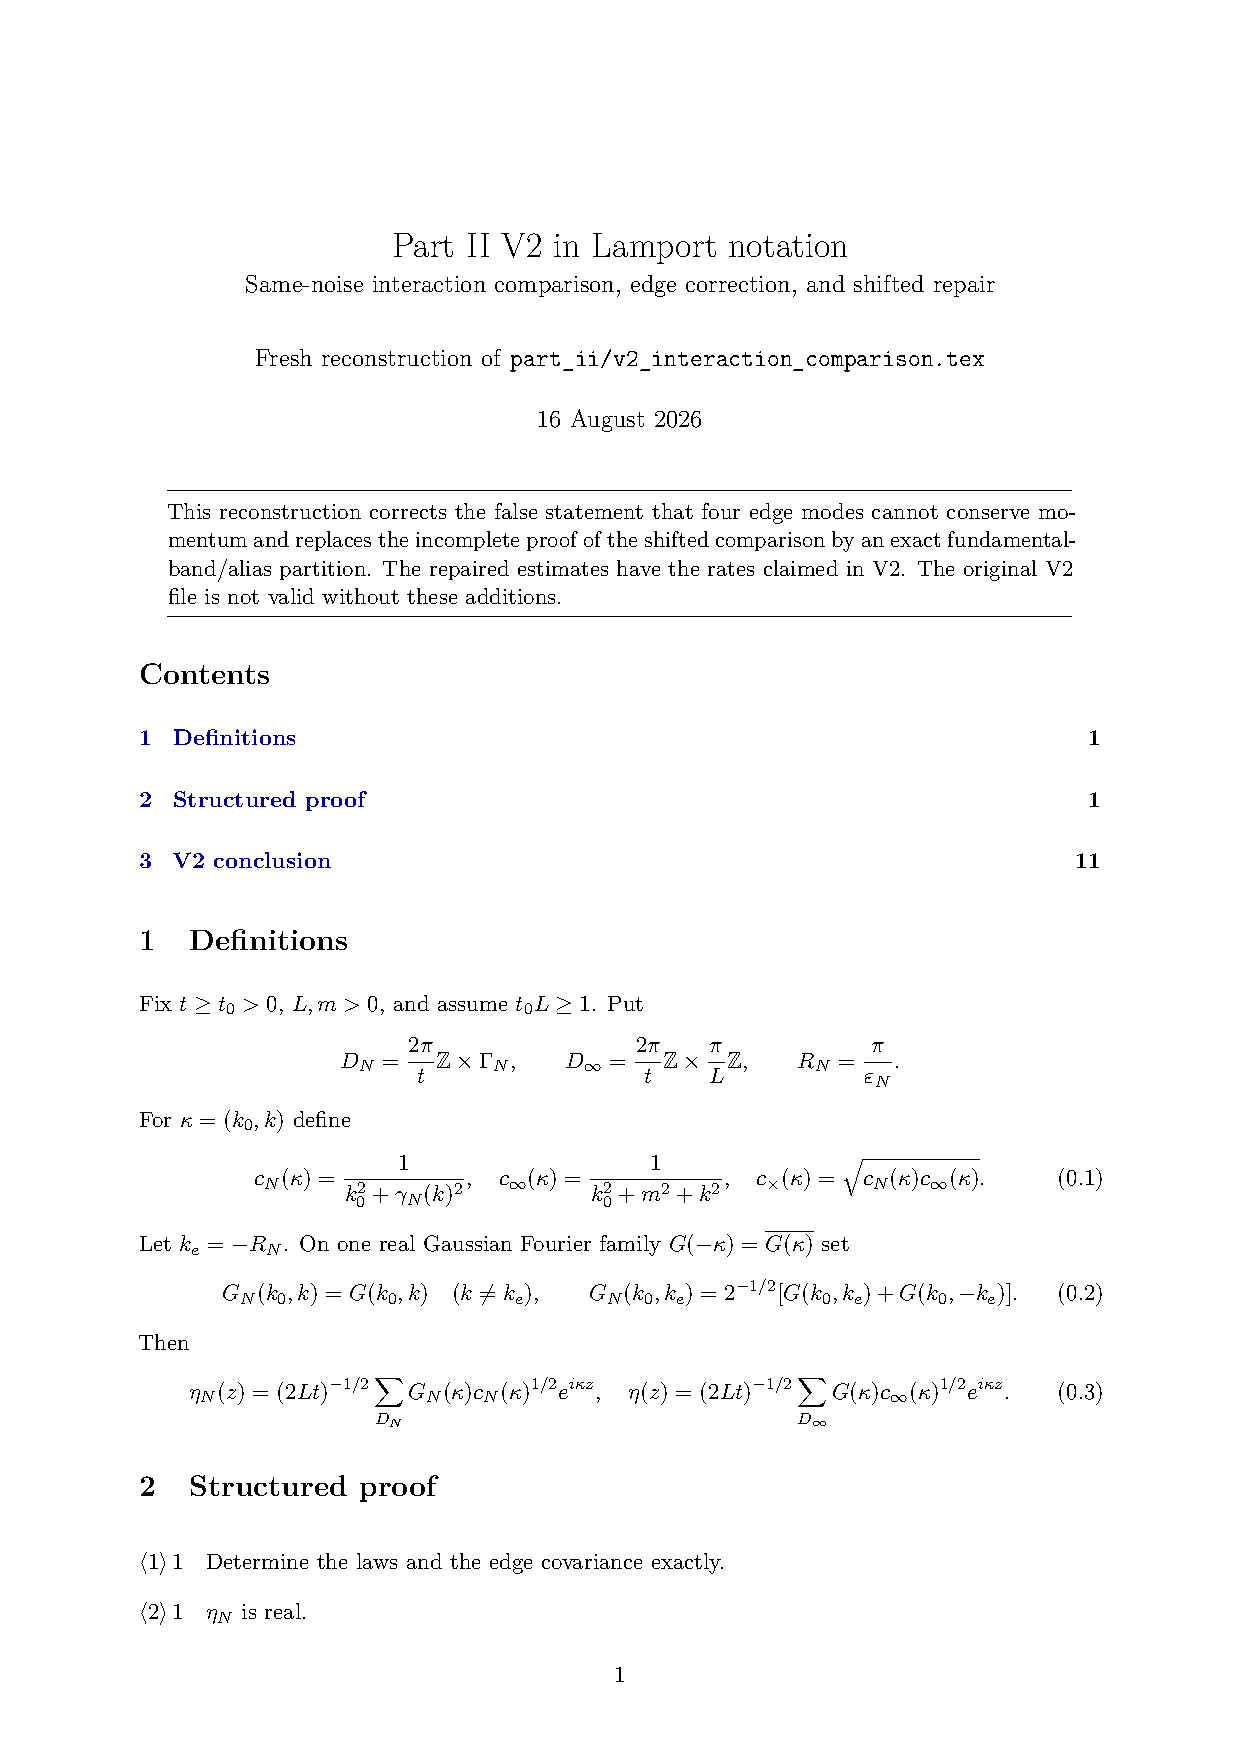
\includepdf[pages=-,pagecommand={\thispagestyle{empty}},addtotoc={1,section,1,
{Part II V2: Interaction comparison and repair},mod:ii-v2}]
{lamport/part_ii_v2_comparison.pdf}

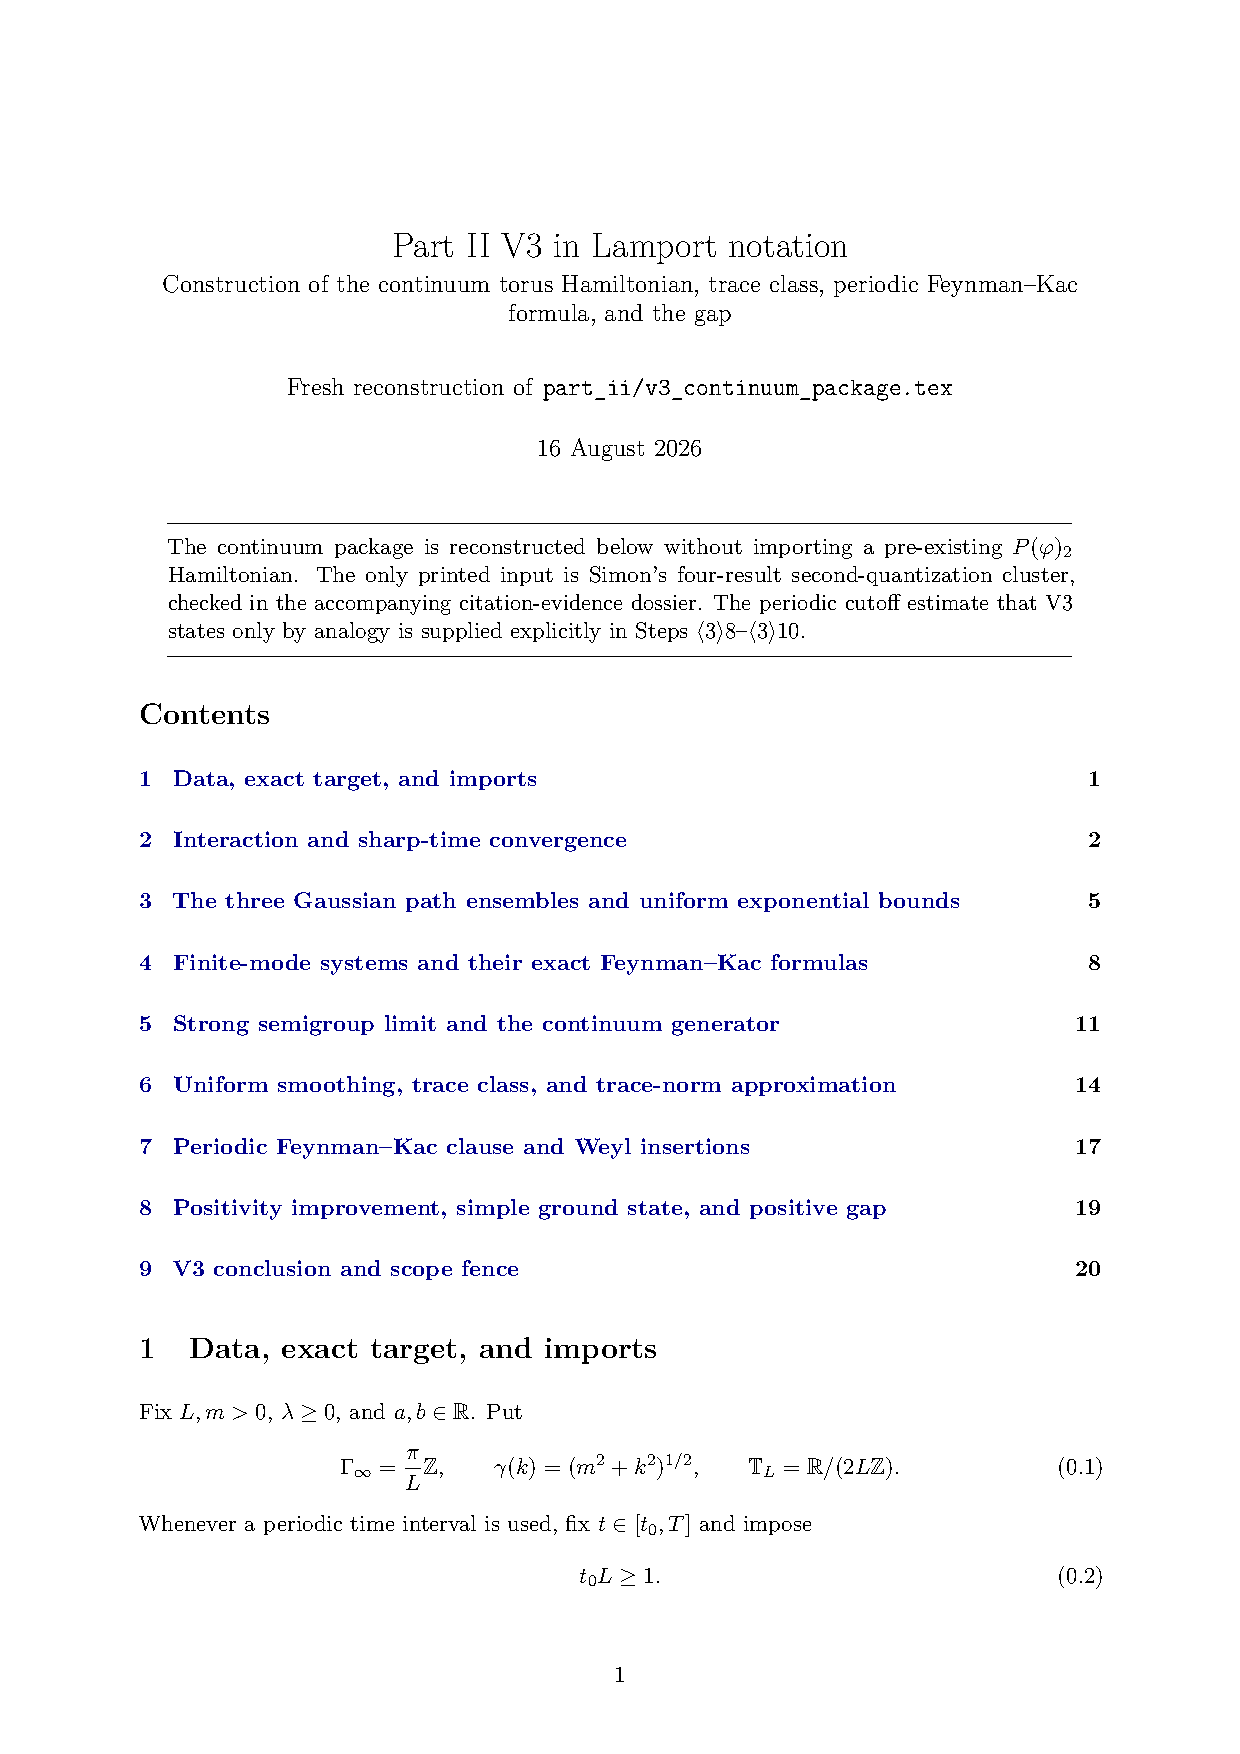
\includepdf[pages=-,pagecommand={\thispagestyle{empty}},addtotoc={1,section,1,
{Part II V3: Continuum package},mod:ii-v3}]
{lamport/part_ii_v3_continuum.pdf}

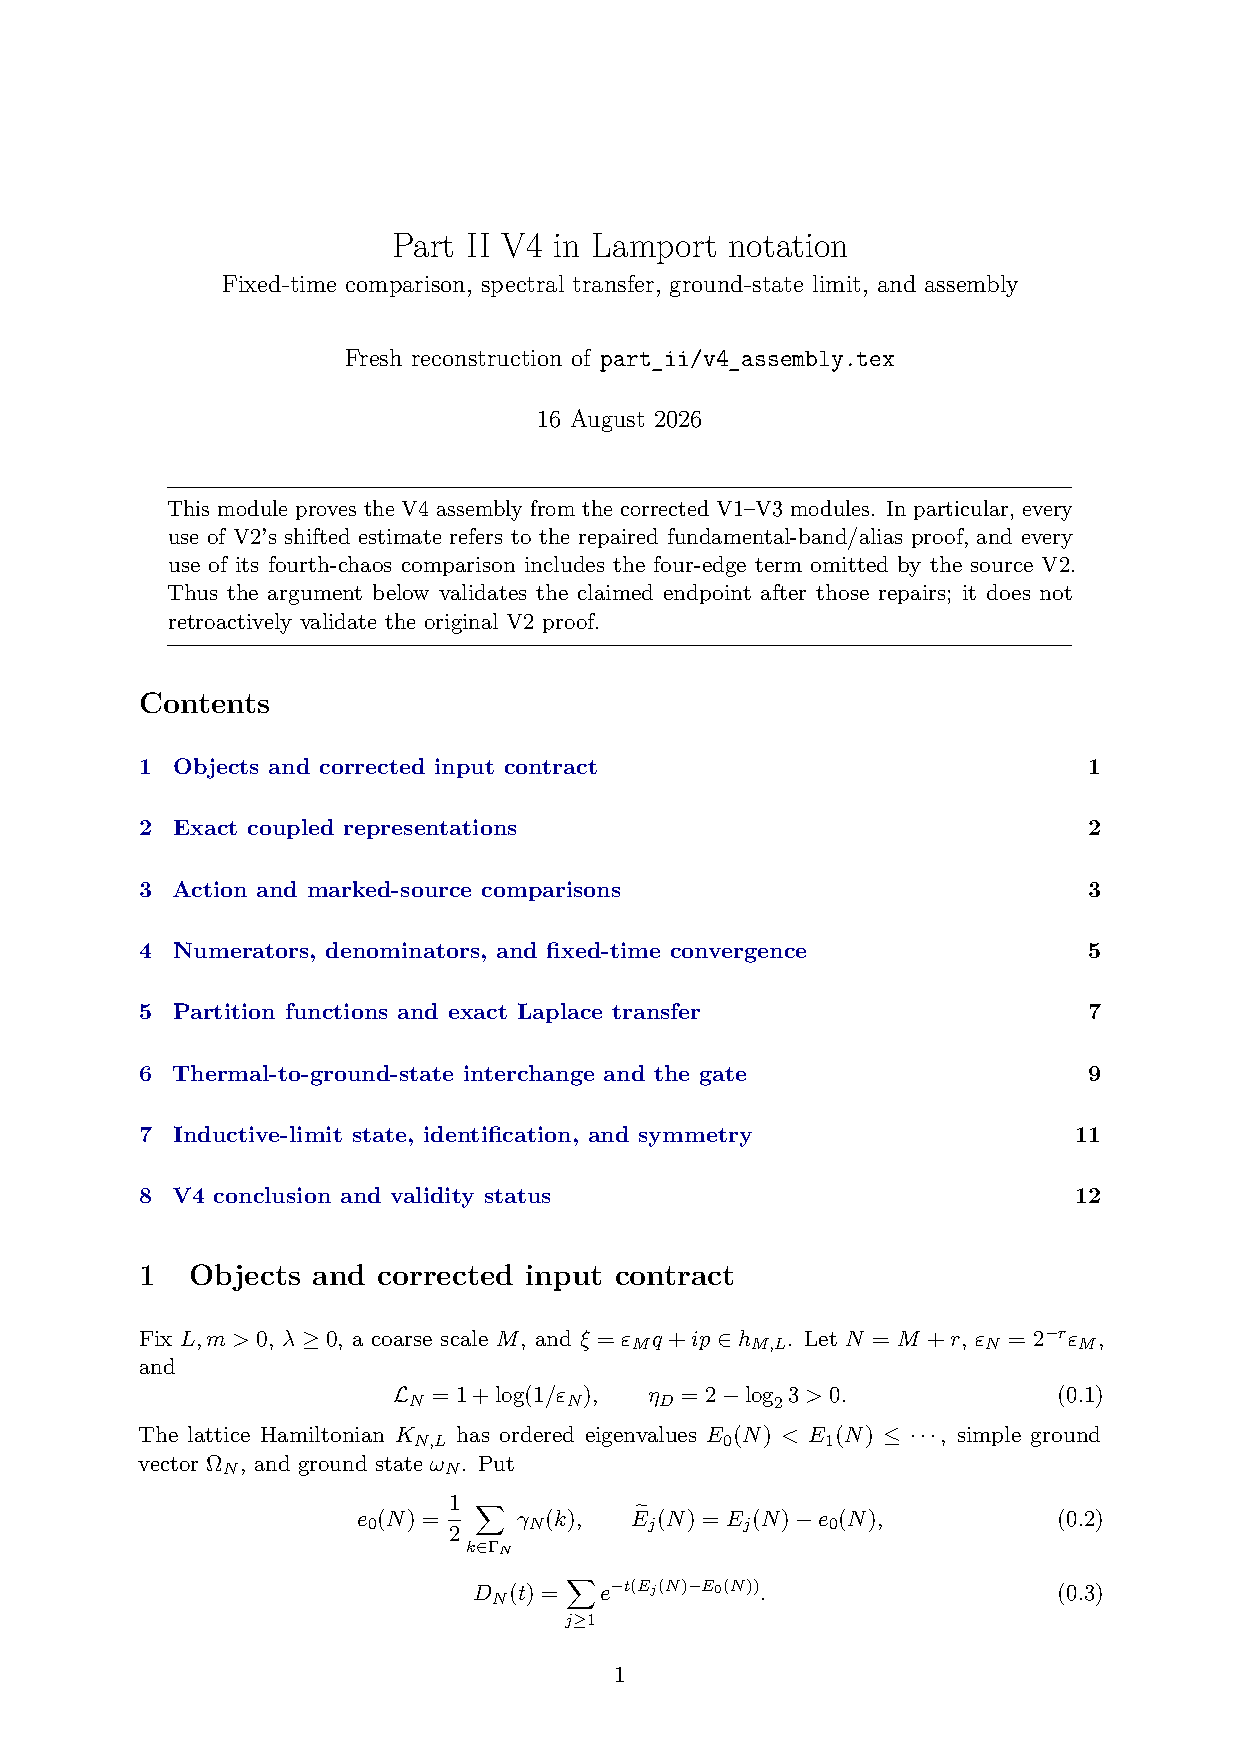
\includepdf[pages=-,pagecommand={\thispagestyle{empty}},addtotoc={1,section,1,
{Part II V4: Assembly},mod:ii-v4}]
{lamport/part_ii_v4_assembly.pdf}

\end{document}
